%%%%%%%%%%%%%%%%%%%%%%%%%%%%%%%%%%%%%%%%%%%%%%%%%%%%%%%%%%%%%%%%%%%%%%%%%%%%%%%%
%2345678901234567890123456789012345678901234567890123456789012345678901234567890
%        1         2         3         4         5         6         7         8


\documentclass[letterpaper, 10 pt, conference]{ieeeconf}  % Comment this line out if you need a4paper

%\documentclass[a4paper, 10pt, conference]{ieeeconf}      % Use this line for a4 paper


\IEEEoverridecommandlockouts                              % This command is only needed if 
                                                          % you want to use the \thanks command

\overrideIEEEmargins                                      % Needed to meet printer requirements.

% See the \addtolength command later in the file to balance the column lengths
% on the last page of the document

% The following packages can be found on http:\\www.ctan.org
%\usepackage{graphics} % for pdf, bitmapped graphics files
%\usepackage{epsfig} % for postscript graphics files
%\usepackage{mathptmx} % assumes new font selection scheme installed
%\usepackage{times} % assumes new font selection scheme installed
%\usepackage{amsmath} % assumes amsmath package installed
%\usepackage{amssymb}  % assumes amsmath package installed
\usepackage{graphicx}
\usepackage{times} % assumes new font selection scheme installed
%\usepackage{amsthm}
\usepackage{amsmath} % assumes amsmath package installed
\usepackage{amssymb}  % assumes amsmath package installed
\usepackage{mathrsfs}
\usepackage[lined,commentsnumbered,ruled]{algorithm2e}
\usepackage{color}
\usepackage{comment}
\usepackage{subfigure}
\usepackage{hyperref}
%\usepackage[dvips,dvipdfm,colorlinks=true,urlcolor=blue,citecolor=blue,linkcolor=blue,bookmarks=true]{hyperref}
\usepackage{multirow}
\usepackage{float}
\usepackage{enumerate}
\usepackage{epstopdf}
\usepackage{array}

\title{\LARGE \bf
A framework for Deploying Multiple Mobile Robots using Topological Maps
}


\author{Albert Author$^{1}$ and Bernard D. Researcher$^{2}$% <-this % stops a space
%\thanks{*This work was not supported by any organization}% <-this % stops a space
\thanks{$^{1}$Albert Author is with Faculty of Electrical Engineering, Mathematics and Computer Science,
        University of Twente, 7500 AE Enschede, The Netherlands
        {\tt\small albert.author@papercept.net}}%
\thanks{$^{2}$Bernard D. Researcheris with the Department of Electrical Engineering, Wright State University,
        Dayton, OH 45435, USA
        {\tt\small b.d.researcher@ieee.org}}%
}


\begin{document}



\maketitle
\thispagestyle{empty}
\pagestyle{empty}


%%%%%%%%%%%%%%%%%%%%%%%%%%%%%%%%%%%%%%%%%%%%%%%%%%%%%%%%%%%%%%%%%%%%%%%%%%%%%%%%
\begin{abstract}

Multi robot deployment problem has been attracted by many researchers in recent years. In this paper we propose a new platform for this problem, in which it is made upon a topological map that will result extremely reduction in computational cost. We consider a group of robot that must be deployed in the environment and service the events inside their corresponding region. In both simulation and experiment we validate the performance of the presented work.
\end{abstract}

%%%%%%%%%%%%%%%%%%%%%%%%%%%%%%%%%%%%%%%%%%%%%%%%%%%%%%%%%%%%%%%%%%%%%%%%%%%%%%%%
\section{INTRODUCTION}

In multi robot systems, one of the fundamental operations is deployment and coverage. The main objective it to obtain the best positions in the work space to put the robots on them, in which robots must have minimum distance to their corresponding region. Therefore, robots can respond to the demands in the minimum time which is the goal of many applications in this area.
Robot deployment has many applications including surveillance and monitoring, rescues operation etc, where a group of robots cover a large area in a cooperative way. 
%

Many researchers have been working in these area to find an efficient and comprehensive solution. In general two types of solutions have proposed for continues and discrete environments. Different method have proposed for different space (convex, non convex), dynamic density function, different metric (Euclidean, geodesic and GVDGeodesic), distributed and centralized etc.
%

But one of the major challenges in all extensions is the computational complexity, since in all of them we need to compute Voronoi region for each robot which cause a lot of calculation to compute the distance of the robot's current position to all points in the region based on a specific metric. Discrete methods have presented a substantial reduction in the computation by discretizing the environment to cells. In this way, as the number of points in the environment is decreased the computation of the total calculation will be less than continues solutions. But it still depends on the metric.
%

In this paper, in order to overcome the important shortage of complexity, we propose a simple but efficient topological map which eliminates all the redundant computation of the previous works. 
%

Our idea is inspired from the human explicit treatment in giving or saving an address. In such a case, human does not need to localize itself precisely, also it is enough to just be informed about the direction and number of turn to get to the desired location. Therefor we present a new topological map given by a graph, in which the robot does not need to find its accurate position in the map. 
%

It should be mentioned that the best environment to have maximum performance of using this idea is in the office like or block based environment. Obviously, the number of offices like building in the governmental offices or big companies, cities in the shape of blocks are not few. Hence our proposed deployment method based on the new topological platform can have a vast usages.
% lower complexity, does not need metric

As the milestones method does not employ any metric, therefore in contrast to the state of the art the computational cost reduce extremely. The other shortcoming that other methods are suffering is the necessity of having precise localization, which makes robot's movement very slowly. In contrast, robot in our method can move as much as speed it can. Arguably, this advantage brings a fast response which might be very vital in application related to delivering. 
% does not need the exact map, an skis is enough

% convergence 
The other contribution that the proposed approach takes into account is the convergence of deployment. In this paper, we show that how a heuristic method proves the convergence of robots movements in the local optimal position in the environment iteratively.

% distributed 
In many applications in real word robots can not be controlled by a centralized system because of the communication limitation. Our method is fully distributed in which each robot need to be contacted just with its neighbors. 
% 
Heterogeneous 
%

{\color{red} density function in a real map can be car traffic.}

%
The organization of this paper is done as following:
section ? is dedicated to 
%
%%%%%%%%%%%%%%%%%%%%%%%%%%%%%%%%%%%%%%%%%%%%%%%%%%%%%%%%%%%%%%%%%%%%%%%%%%%%%%%%
\section{Related work}

Multi robot coverage and deployment have recently received a great deal of attention due to the applicability as a fundamental tools in different real work application.
%
Among such previous approaches, different classification can be defined: distributed and centralized; continues and discrete.
%
In the distributed approaches, robots are equipped with sensors and they have the ability to make their decision based on the captured information from the environment. Such a system, is useful where the robots can not communicate to each other frequency.
%
In contrast, in a centralized system a group of robots are controlled by a central system which has communication to them.
%
\\
Deployment in a discrete model of the environment proposed to not only improve the computational cost of the continues models, but also because of the nature of the discrete applications. In continuation of our reviewing, we explain some of the literature in these two categories.
%

Cortes \cite{Cortes2004}
%
safety \cite{reza2014}
%
\cite{Stergi2011}
%
% ===========================================
deployment problem
%
%Continues 
The  work in this area was proposed by Cortes \cite{Cortes2004} based on Lloyd framework for optimized quantization \cite{Lloyd1982}. In 

Afterwards, many researchers have improved his work on the different aspect, for instance in \cite{Pimenta2008}, \cite{Breitenmoser2010}, \cite{Stergi2011}, \cite{Tzes2010}, \cite{Mahboubi2012}, \cite{Yun2013}, \cite{Durham2012}. \cite{Bhattacharya2013a}

These works were limited to a convex environment with smooth sensory functions.
•	?? propose a bionomic heuristic, and in a later work, ?? present an algorithm based on a set partitioning formulation.

%
Discrete 
%
graph based
\cite{Yun2013}

p median problem 

%%%%%%%%%%%%%%%%%%%%%%%%%%%%%%%%%%%%%%%%%%%%%%%%%%%%%%%%%%%%%%%%%%%%%%%%%%%%%%%%
\section{Problem definition}

In this paper we address a well-known multi robot deployment problem, in which the objective is to find the best location of each robot in its dedicated partition of an environment. We also propose a new platform based on a topological map which is a simple representation of an environment like a topological graph. Hence, we modify the standard deployment problem to be applicable in this topological map. Furthermore, to be able to use this kind of map, we assume that the environment contains symmetric corridors and intersections like many public and governmental buildings: hospitals, universities departments, supermarkets etc. Therefore, robots will move within these corridors to find the best configuration to be deployed. An example of this type of map is depicted in Fig. \ref{fig:samplemap}

\begin{figure}[h]
\centering
	\subfigure[A map of a building contains corridors and intersections.]{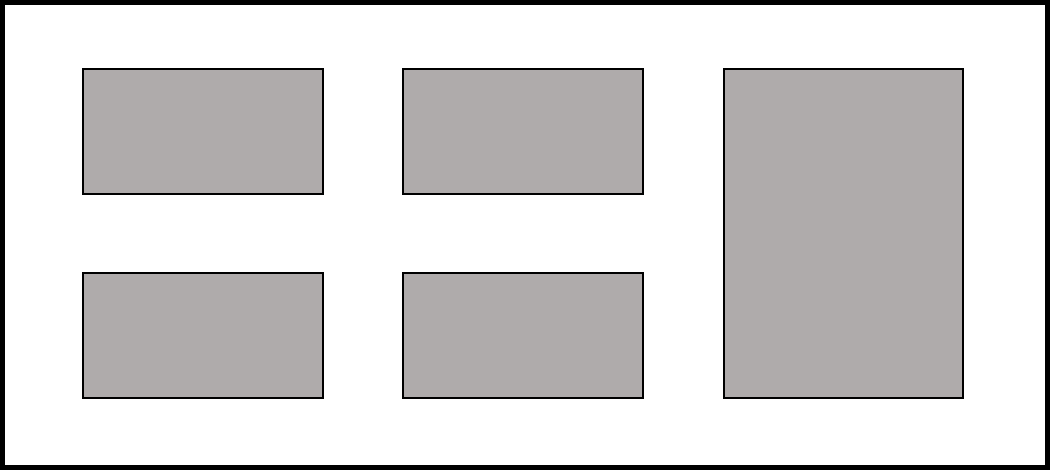
\includegraphics[width=1\columnwidth]{Figures/SampleMap2.png}} \\
    \subfigure[Corresponding nodes area.]{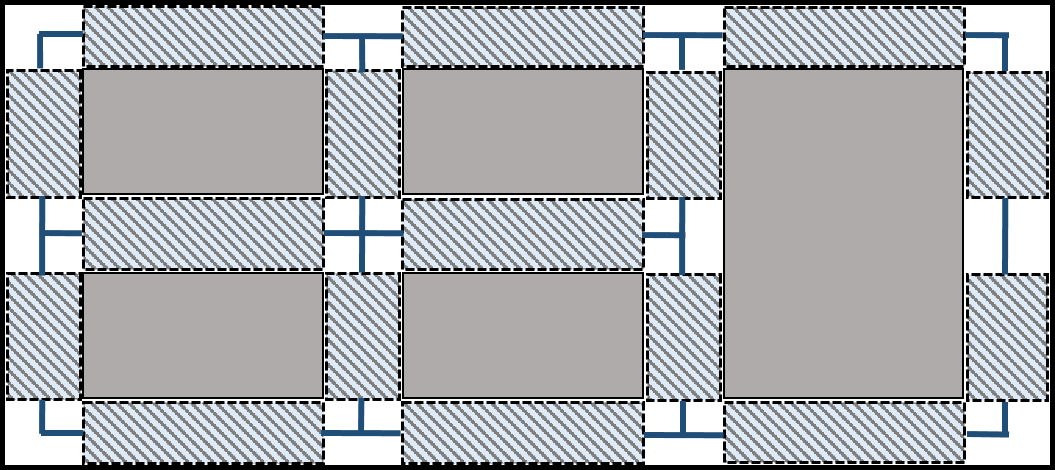
\includegraphics[width=1\columnwidth]{Figures/SampleMapWithGraph2.png}} \\
    \subfigure[Corresponding graph.]{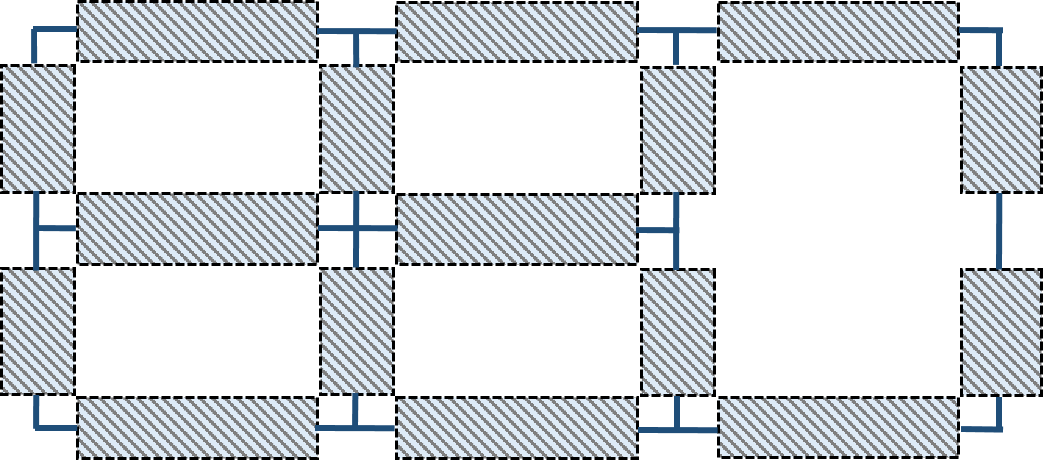
\includegraphics[width=1\columnwidth]{Figures/SampleGraph2.png}}    
    \caption{A sample map with the corresponding graph representation.}
    \label{fig:samplemap}
\end{figure}

% topological map
In this figure, the gray regions indicate rooms and white corridors are the region where robots will move in. To address the navigation of robots in this workspace, we assume robots are equipped by a planar laser range finder to detect walls of the corridor, intersections, people, and other obstacles in the environment. This ability can be considered as a milestone in robot navigation, since it facilitate the implementation of the robot control without need of odometery sensors.
%
The utility of this platform manifests in different applications, for instance consider a service robot can quickly navigate through this kind of workspace might be used to make deliveries, to guide visitors, or even to guard the building.

Based on this platform, the multi robot deployment problem can be defined as follows:

% deployment problem
Given a bounded environment, $\Omega \subset \mathbb{R}^2$, let $P=\{p_1, . . . , p_n \}$ denote the configuration of $n$ robots, $N=\{1, . . . , n\}, n \in \mathbb{N}$ indicated to the set of robots, and $V_i$ Voronoi region in $\Omega$ is defined as:

\begin{equation}
\label{eq:VoronoiregionCVT} V_i = \{\mathbf{x} \in \Omega |
||x-p_i|| \leq ||x-p_j||, \forall j
\in N\}, i \in N, i\neq j.
\end{equation}

Region $i$ the region that robot $i$ is associated to this region, and $\cup_{i=1}^n V_i=\Omega$. 
All points $x\in \mathbb R^2$ that lie in the interior of any $v_i$ are considered to be surveyed by the robot $i$.

\textit{locational deployment folrmulation} is given by  \cite{Cortes2004}:
:

\begin{equation}\label{eq:functional1}
\mathcal{H}(P, V) = \sum_{i=1}^{n}\mathcal{H}(\mathbf{p}_i,V_i)=
\sum_{i = 1}^{n} \int_{V_i}
d(\mathbf{q},\mathbf{p}_i)\phi(\mathbf{q})d\mathbf{q} \,,
\end{equation}


%%%%%%%%%%%%%%%%%%%%%%%%%%%%%%%%%%%%%%%%%%%%%%%%%%%%%%%%%%%%%%%%%%%%%%%%%%%%%%%%

\section{Methodology}



%topological graph
\begin{figure}[H]
\centering
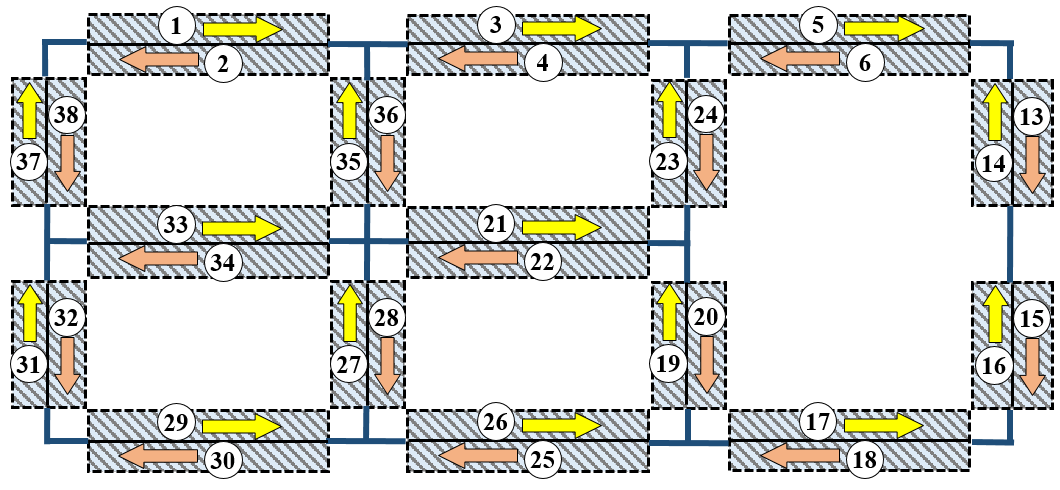
\includegraphics[width=1\columnwidth]{Figures/SampleGraphNumbered2.png}
\caption{A graph with numbered nodes.}
\label{fig:numbedGraph}
\end{figure}

%new H function

%%%%%%%%%%%%%%%%%%%%%%%%%%%%%%%%%%%%%%%%%%%%%%%%%%%%%%%%%%%%%%%%%%%%%%%%%%%%%%%%
\section{Implementation result}
%
\subsection{Simulation results}
%
For the simulation we select a real map of a neighborhood in New York city from Google Maps (See Fig. \ref{fig:googlemap})
%
\begin{figure}[H]
	\centering	
	\subfigure[Sattelite view.]{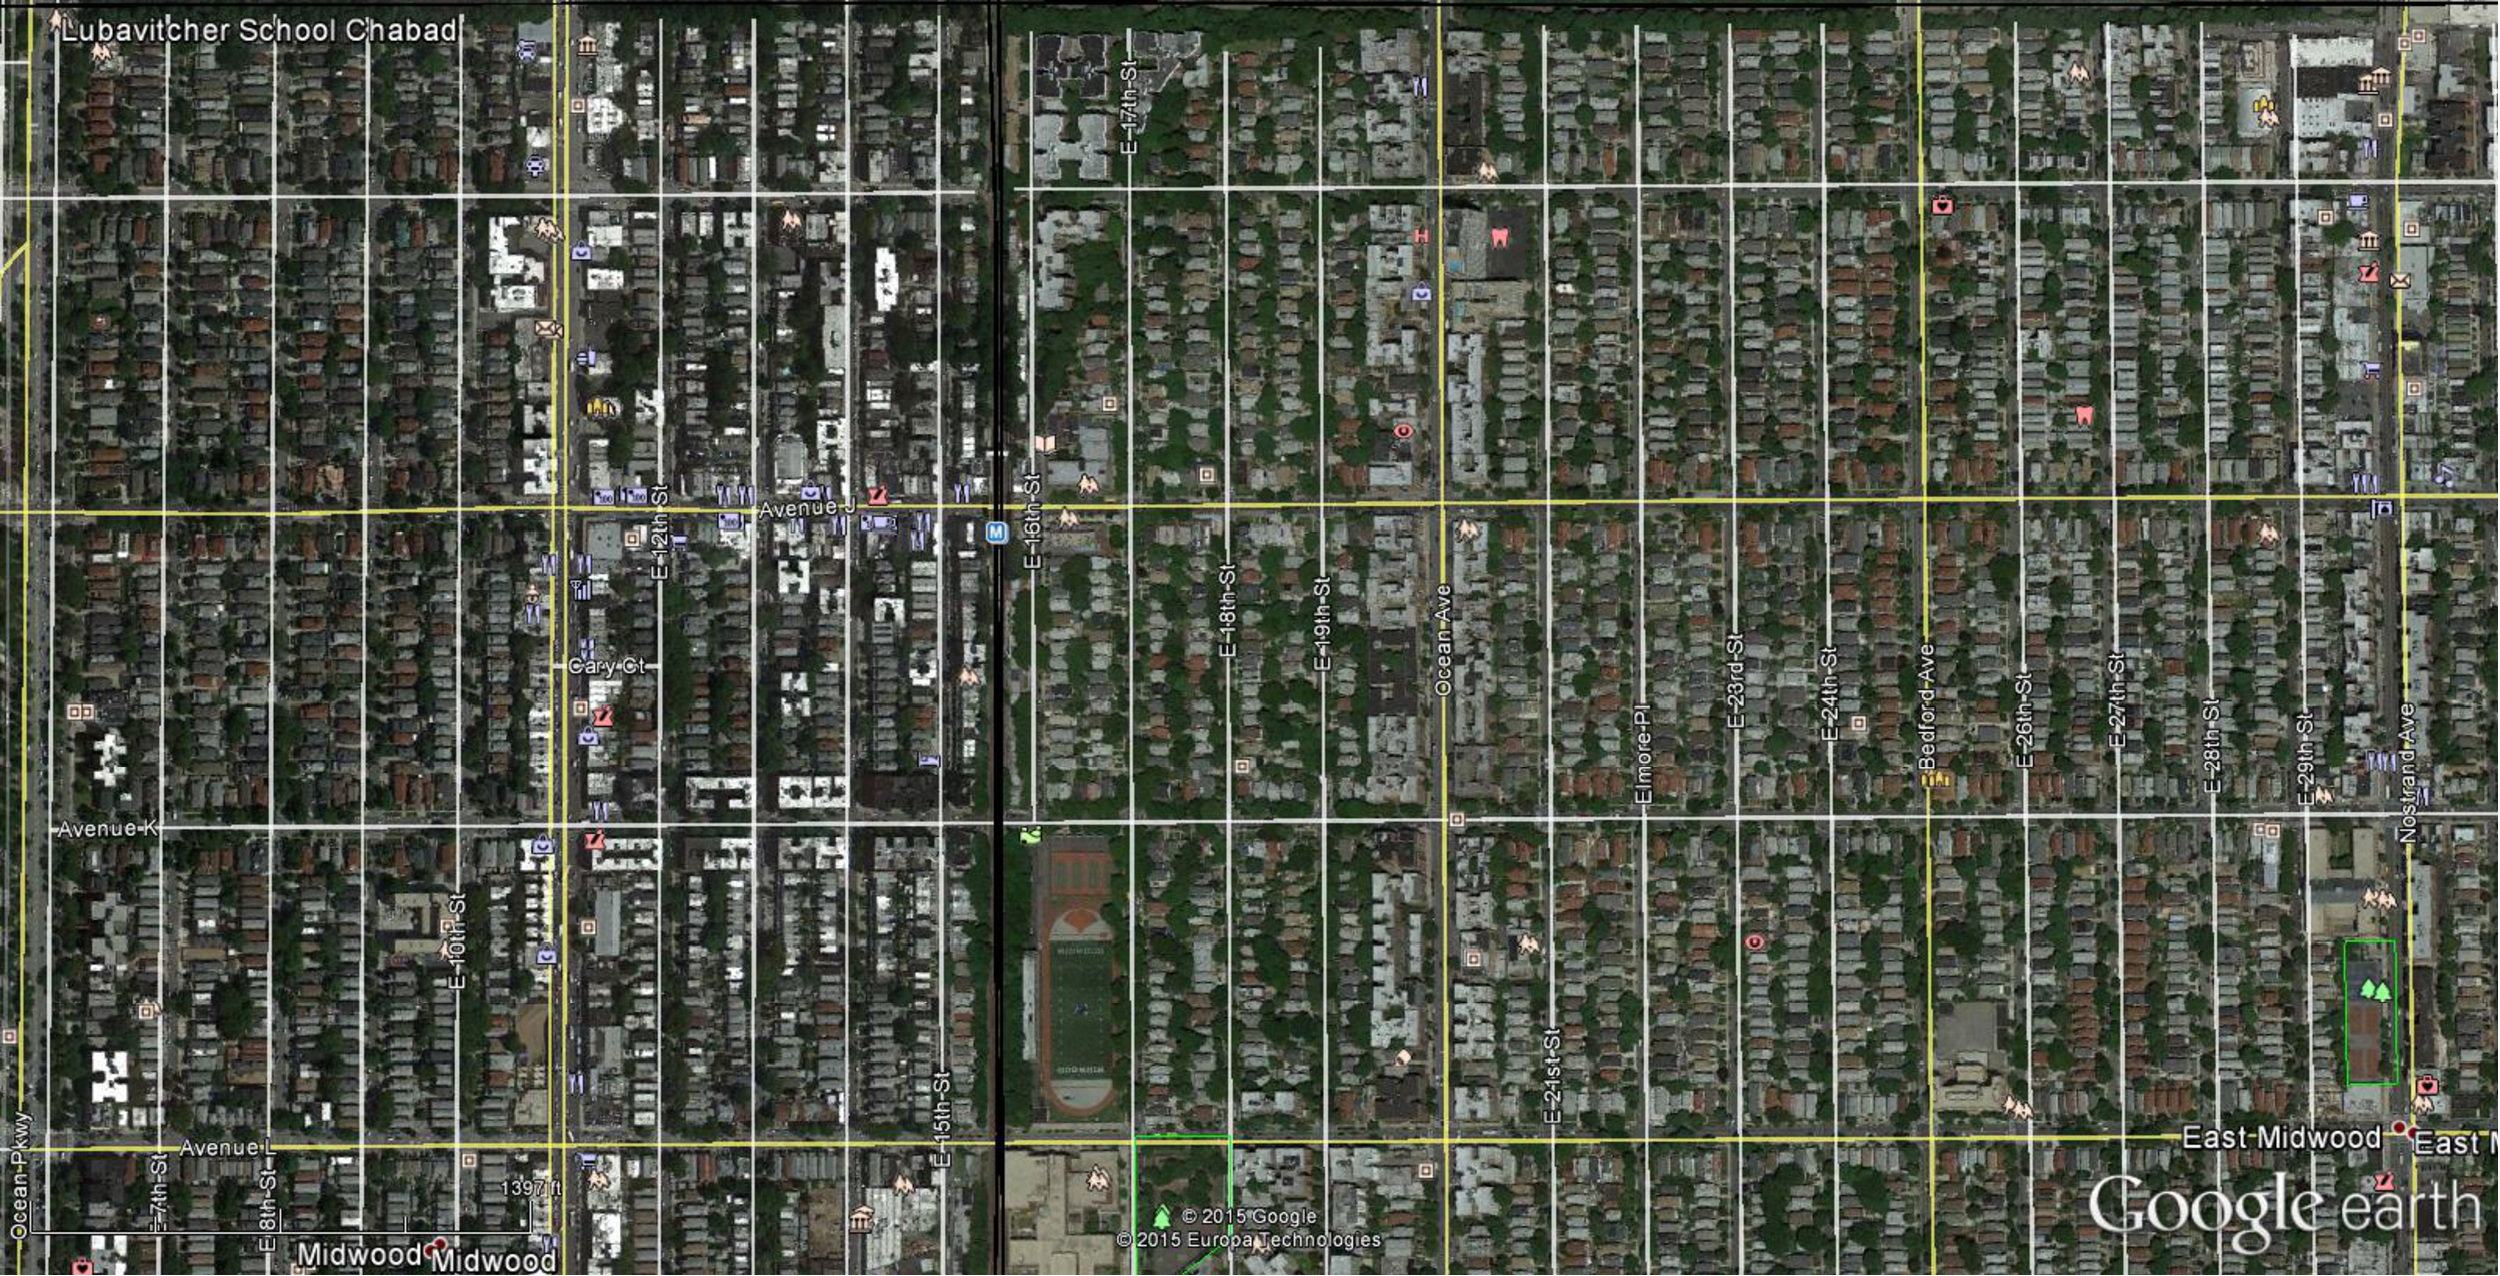
\includegraphics[width=1.0\columnwidth]{Figures/map4lables.pdf}}
	\subfigure[Corresponding binary image.]{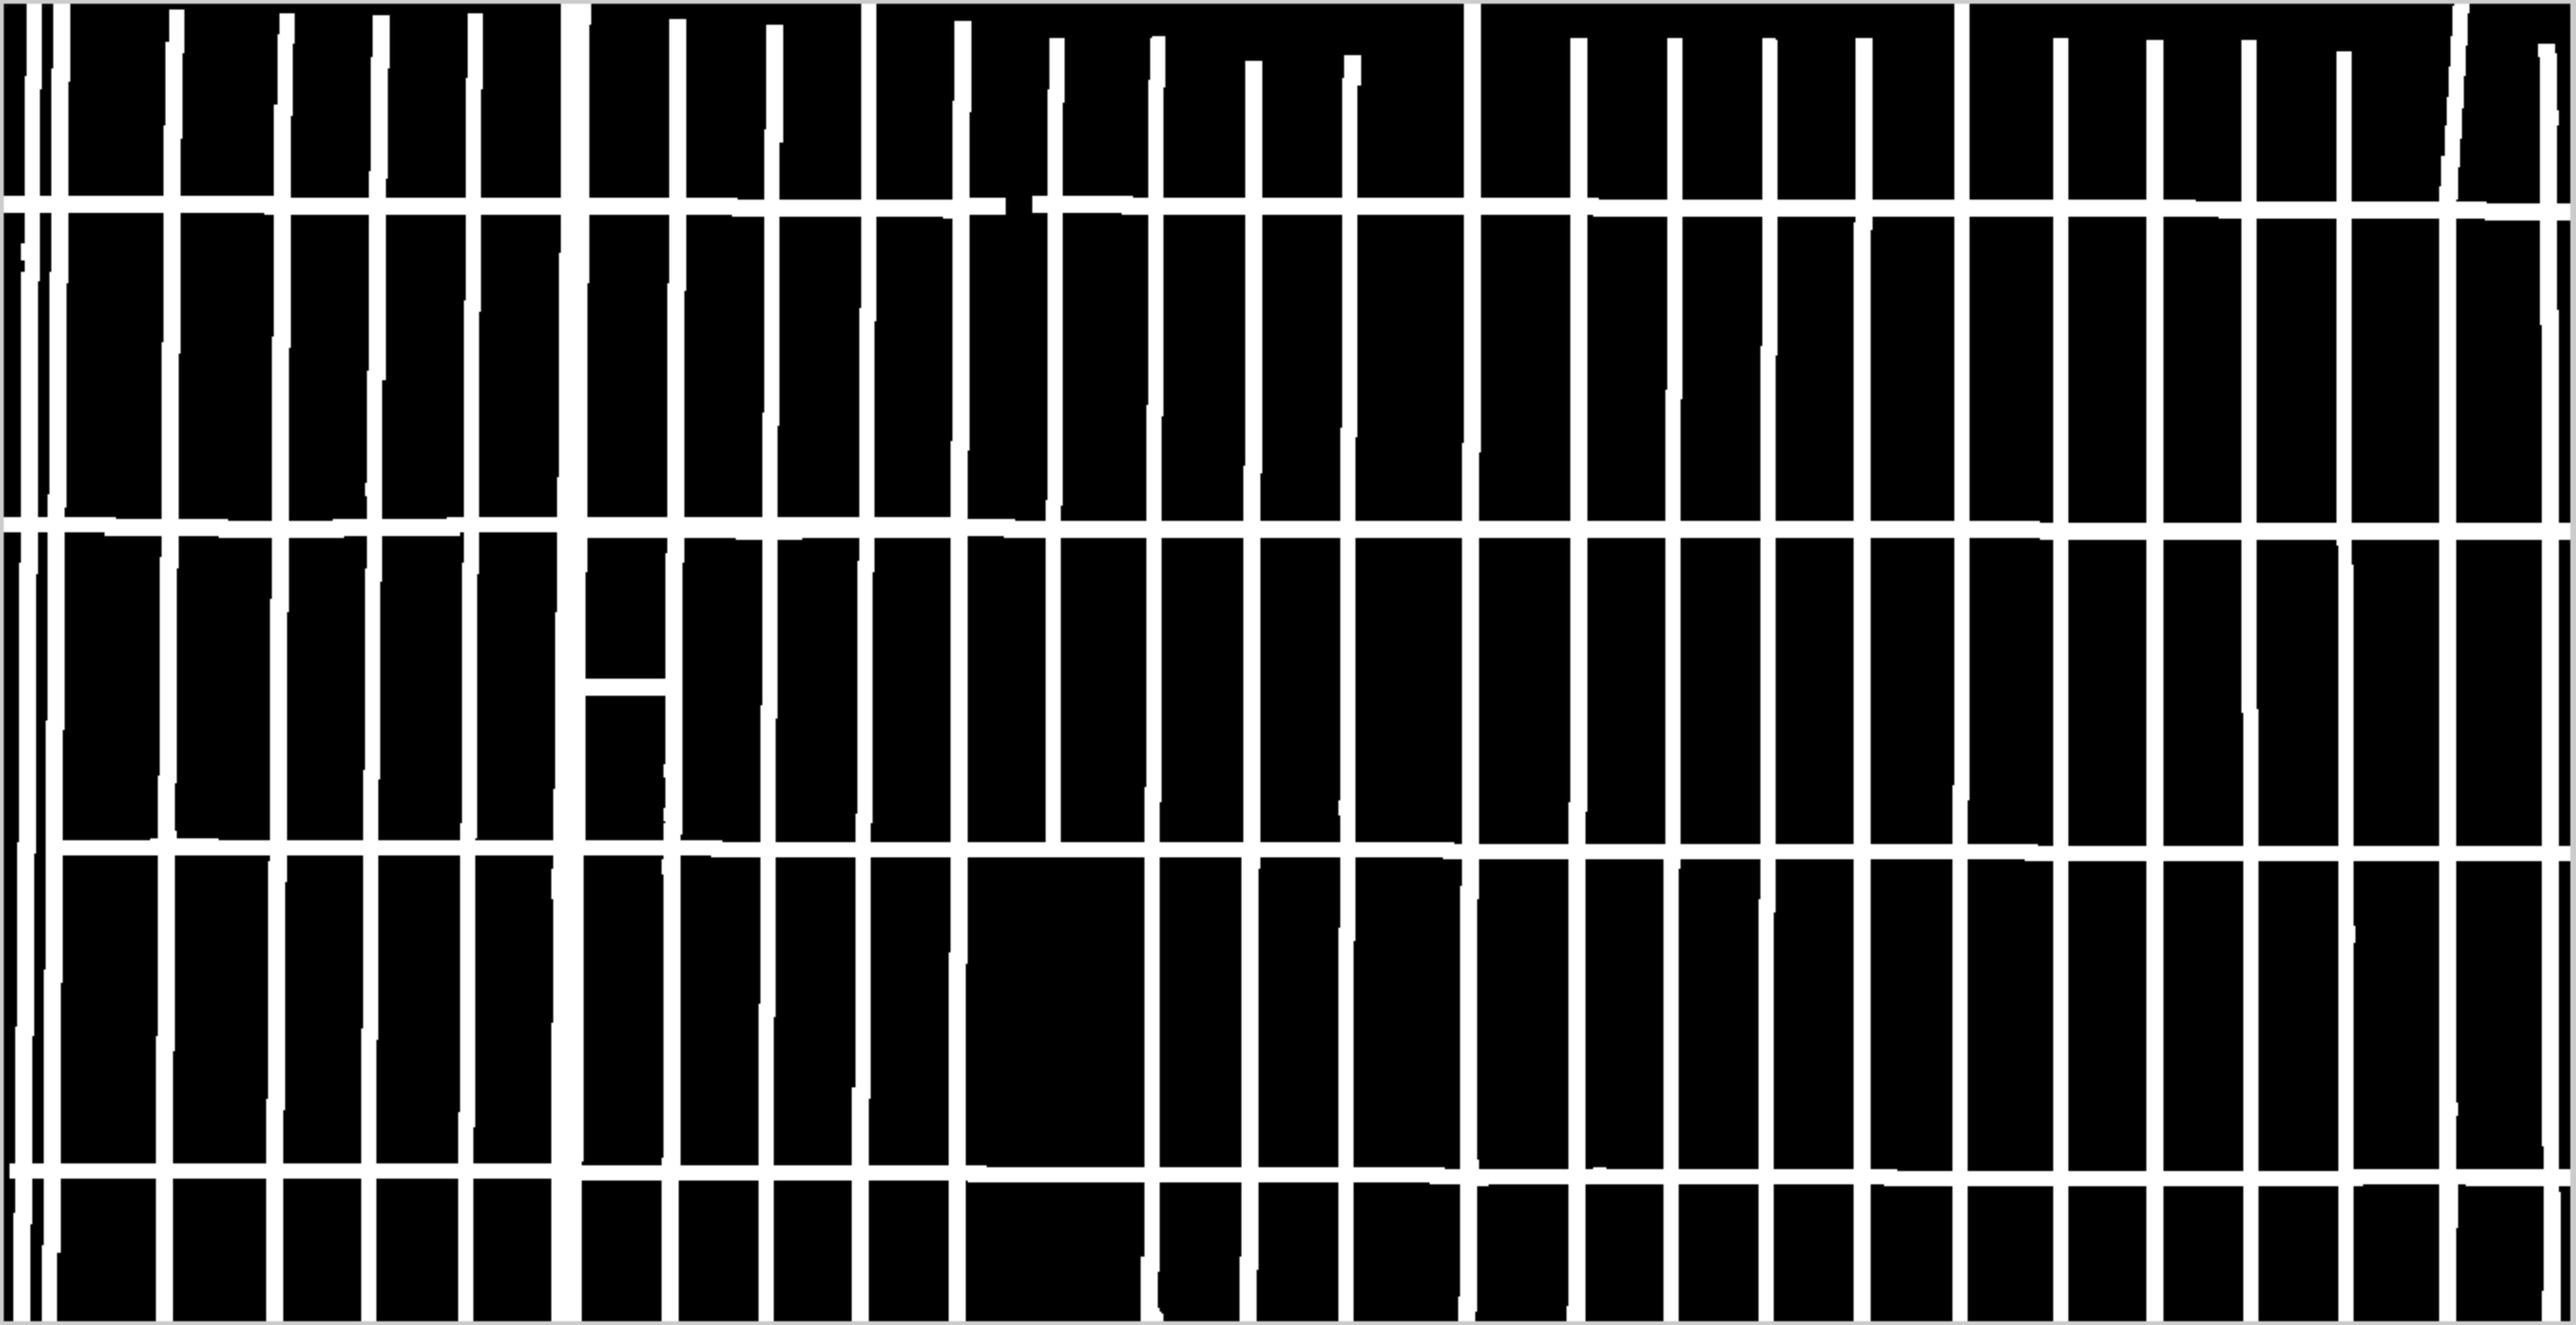
\includegraphics[width=1.0\columnwidth]{Figures/googlemapGVD.pdf}}
	\caption{A map grabbed from Google map.}
	\label{fig:googlemap}
\end{figure}
%

\subsection{Real robot experiments}
%
with 4 real robots
%%%%%%%%%%%%%%%%%%%%%%%%%%%%%%%%%%%%%%%%%%%%%%%%%%%%%%%%%%%%%%%%%%%%%%%%%%%%%%%%
\section{CONCLUSIONS}
%


%%%%%%%%%%%%%%%%%%%%%%%%%%%%%%%%%%%%%%%%%%%%%%%%%%%%%%%%%%%%%%%%%%%%%%%%%%%%%%%%
\section*{APPENDIX}

Appendixes should appear before the acknowledgment.

\section*{ACKNOWLEDGMENT}

CAPES, CNPq, UFMG...



%%%%%%%%%%%%%%%%%%%%%%%%%%%%%%%%%%%%%%%%%%%%%%%%%%%%%%%%%%%%%%%%%%%%%%%%%%%%%%%%

\bibliographystyle{IEEEtran}
\bibliography{Mendeley} 



\end{document}